\section{Electrical Design}
MAVEN-01 is designed to be an affordable autonomous vehicle platform for research and educational purposes, so
as we chose low range price electrical components but still make sure the rover has solid performance by price.

\vspace{1em}
\text{Power source}
We use two 6C 18650 lithium batteries as the main power source for most of the system, include motor, sensors and lights.
Lithium battery always has better power capacity and can be recharged. Two 6C 18650 batteries provide total 7.4V and 13A, which
more than enough for the whole system requirement. 

\vspace{1em}

\textbf{Motor Electrical Diagram}

\begin{figure}[H]
    \centering
    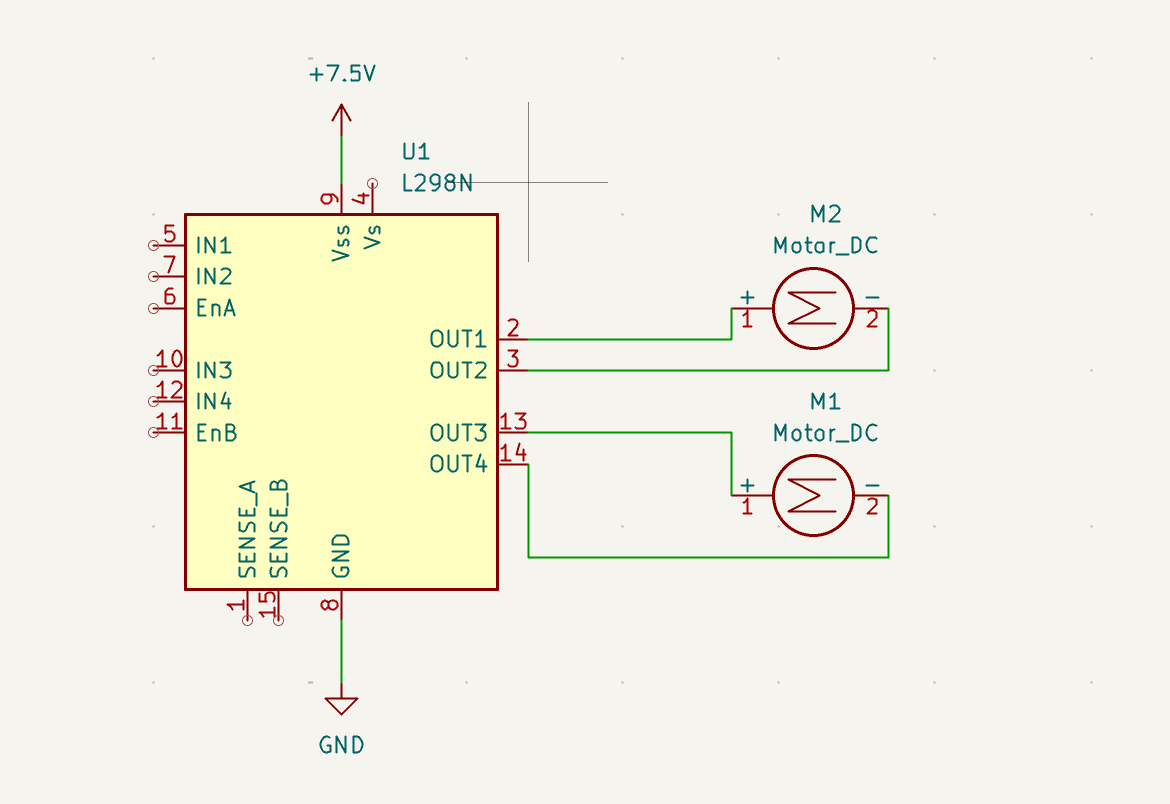
\includegraphics[width=\linewidth]{images/diagram/tt_motor_l298.png}
    \caption{Diagram of connections between L289N with 2 6V TT gear motors}
    \label{fig:l298n_2_motors}
\end{figure}

\vspace{1em}

\par
Two TT motor consume of total 6V due to the parallel wiring method through L298N, this motor driver 
allow power input in range from 5V to 12V, the maximum current <=2A, which are enough for two gear motors with total 
maximum current consume are ~600mA. All calculation follow the Ohm's law, parallel connected module share constant voltage 
with cumulative currents. 

\textbf{Ohm's law}
\[
V = IR
\]

\textbf{Total current of parallel gear arrangement}
\[
I_{\text{total}} = I_1 + I_2 + \cdots + I_n 
\]


\begin{figure}[H]
    \centering
    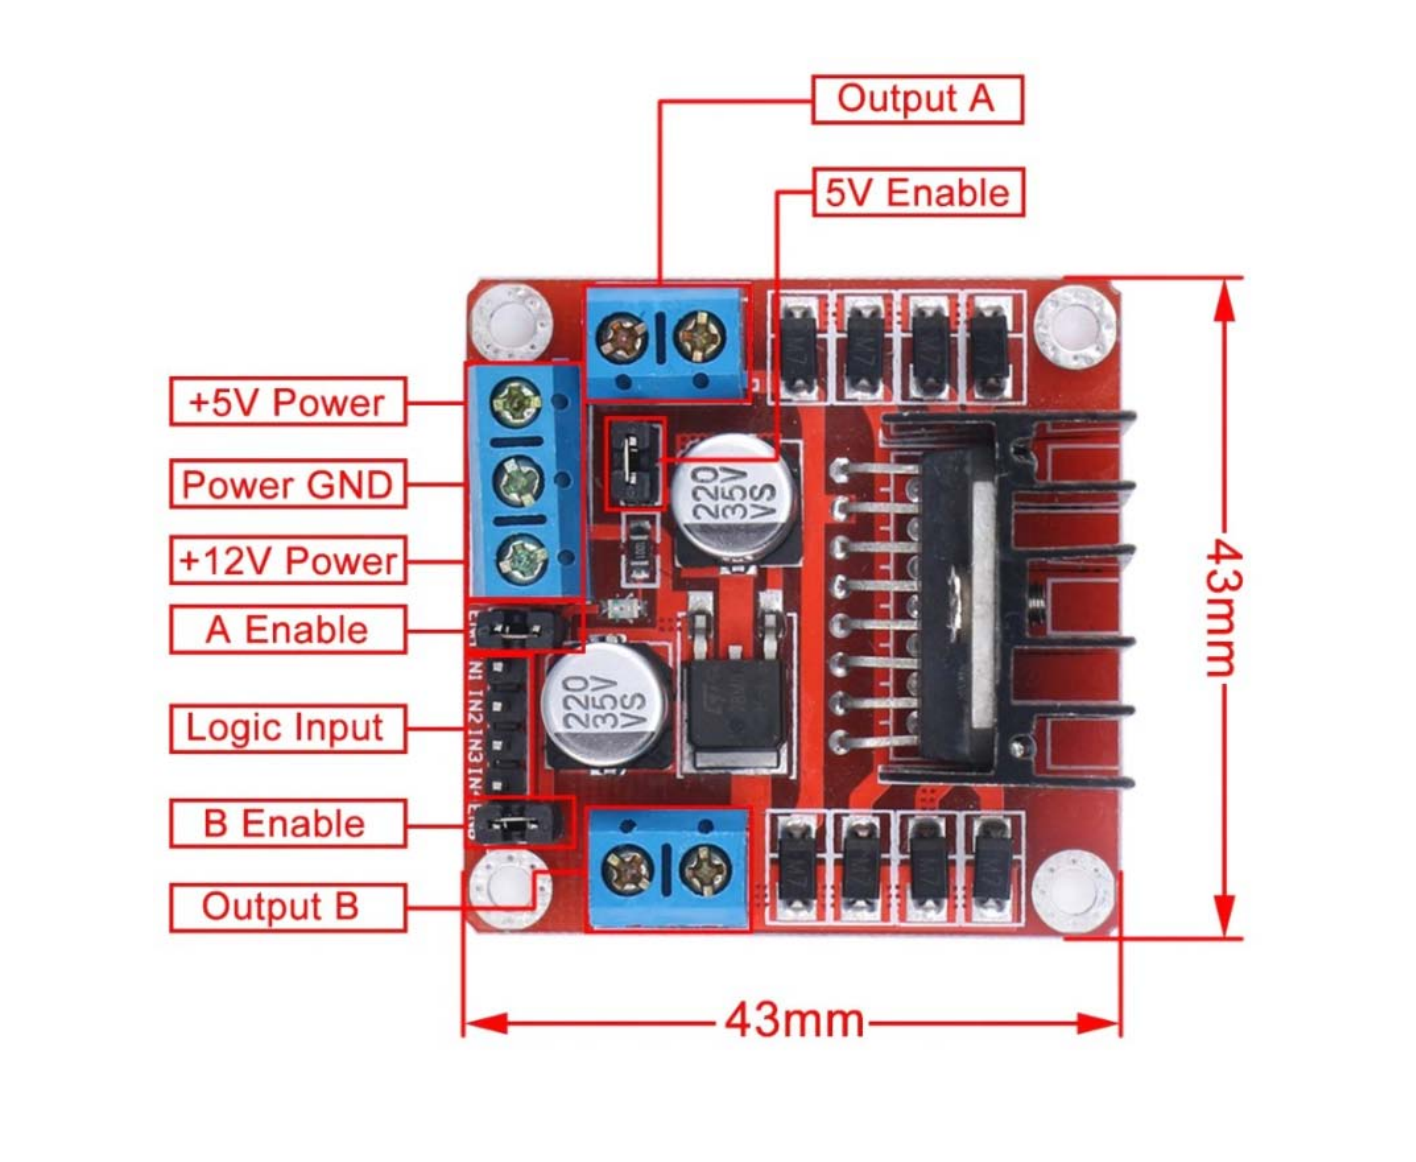
\includegraphics[width=0.8\linewidth]{images/electrical_schematics/L298N_image.png}
    \caption{L298N H-bridge DC motor driver }
    \label{fig:l298n_image}
\end{figure}


\begin{figure}[H]
    \centering
    
\includegraphics[width=0.9\linewidth]{/Users/nguyenthanhvinh/Documents/Papers/reference/final_maven_01_thesis/images/electrical_schematics/L298N.png}
    \caption{Schematic Diagram of L298N H-bridge DC motor driver }
    \label{fig:l298_schematic}
\end{figure}



\begin{figure}[H]
    \centering
    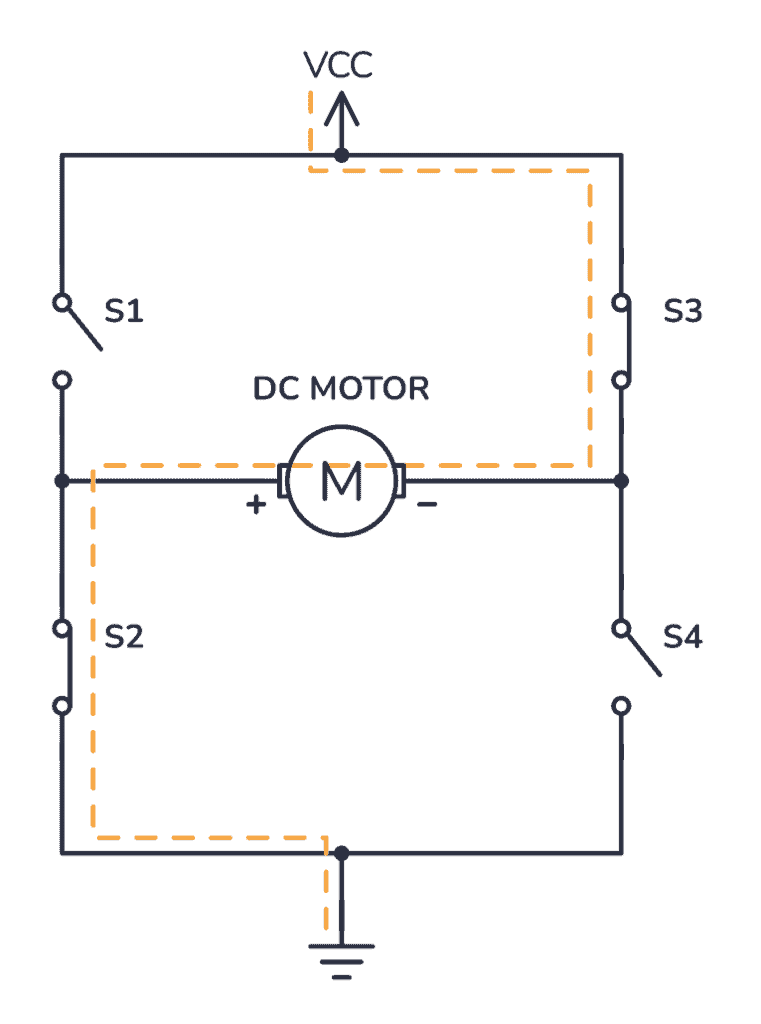
\includegraphics[width=0.5\linewidth]{images/electrical_schematics/h_bridge.png}
    \caption{Schematic Diagram of L298N H-bridge DC motor driver }
    \label{fig:h_bridge_image}
\end{figure}




L298N has a structure called an H-bridge, which allows it to have a total of 4 cases of current direction to control DC motors. 
In Figure~\ref{fig:h_bridge}, we can see an example of a single motor in an H-bridge circuit. 
When \verb|S3| and \verb|S1| are closed, it allows DC current to run through the motor, making it spin counterclockwise. 
On the other hand, if \verb|S1| and \verb|S4| are closed while \verb|S3| and \verb|S2| are open, DC current will run through and make the motor spin in the clockwise direction. L298N has two H-bridge circuits, which in theory can control more than 2 DC motors, as long as the current limit is not exceeded.

\vspace{1.5em}
\par
During the development process, we tested with 1 and 2 DC motors on each bridge and concluded that the L298N can handle 4 DC motors with a total current of approximately 1.2A. 
However, the movement capability will be similar to using 2 motors since the L298N only has 2 H-bridges.
 For better control and manipulation, we decided to switch to a 4-channel motor driver module.

\subsection{Control Protocol}

MAVEN-01 was designed to be teleoperated, so it needs a control board that has some kind of wireless send-and-receive mechanism.
Most of the time, radio signal is the first choice because of its wide range, stable connection, and relatively low power consumption.
However, complete radio control requires a full set including a remote control, transmitter, receiver, etc., which increases the overall cost significantly.

\vspace{1.5em}
In our project, we choose Wi-Fi as the main method to control the rover, not only for control but also to receive data from sensors attached to the rover. 
Because MAVEN-01 is designed for research purposes, Wi-Fi is a better choice. We only need a Wi-Fi built-in microcontroller board such as ESP32 or ESP8266. 
Sensor data are usually complex, so they require a high-bandwidth and low-latency signal to transmit. In this case, Wi-Fi performs better than radio, but the trade-off is higher latency 
and power consumption due to the higher frequency compare to normal radio signal.

\vspace{1.5em}


\subsection{Control Unit: WEMOS D1 R32 (ESP32 based)}
ESP32 is a microcontroller board with built-in WiFi and Bluetooth that we chose as the main control unit.
With its integrated WiFi module, it enables wireless control and sensor data transmission.
Compared to other boards such as Arduino UNO R4 or ESP8266, ESP32 offers faster processing speed and more GPIO pins, 
allowing more sensors to be connected. It is also affordable.

\vspace{1.5em}\par
\textbf{Board Comparison}

\begin{table}[h]
\centering
\begin{tabular}{|l|c|c|c|}
\hline
\textbf{Feature} & \textbf{ESP32} & \textbf{Pico W} & \textbf{UNO R4} \\
\hline
CPU & Dual-core 240 MHz & Dual-core 133 MHz & 48 MHz Cortex-M4 \\
\hline
RAM & 520 KB & 264 KB & 32 KB \\
\hline
Flash & 4 MB & 2 MB & 256 KB \\
\hline
WiFi & Yes & Yes & Yes \\
\hline
Bluetooth & Yes & No & No \\
\hline
GPIO & $\sim$30 & 26 & 14 \\
\hline
RTOS & Yes (FreeRTOS) & No & No \\
\hline
Power & Medium & Low & Low \\
\hline
Price (VND) & $\sim$120k & $\sim$180k & $\sim$700k--1M \\
\hline
\end{tabular}
\caption{Comparison of ESP32, Pico W, and Arduino UNO R4 WiFi}
\end{table}

ESP32 has many variants suitable for specific tasks. 
It also supports camera modules such as OV2640 or OV5640 for video streaming, making it suitable as an FPV camera for the rover.
In MAVEN-01, we used an Arduino-based ESP32 board called \href{https://handsontec.com/dataspecs/module/ESP/WeMos%20D1%20R32.pdf}{WEMOS D1 R32}. 
This board uses the same dual-core processor and features as the standard ESP32 from \href{https://www.espressif.com/}{Espressif}, 
but is easier to use due to its Arduino-like form factor.


\begin{figure}[H]
    \centering
    \includegraphics[width=\linewidth, page= 6]{images/electrical/d1_r32.png}
    \caption{Wemos D1 R32 pins maps, more information about detailed pinout description in \href{https://documentation.espressif.com/esp32-wroom-32d_esp32-wroom-32u_datasheet_en.pdf}{here}}
    \label{fig:chasis_1_engine_blueprint}
\end{figure}



\newpage
\subsection{Temperature ana humidity sensor: DHT11}
\par
\textbf{Overview}
\vspace{1em}

DHT11 Temperature \& Humidity Sensor features a temperature \& humidity sensor
complex with a calibrated digital signal output. By using the exclusive digital-signal-acquisition
technique and temperature \& humidity sensing technology, it ensures high reliability and
excellent long-term stability. This sensor includes a resistive-type humidity measurement
component and an NTC temperature measurement component, and connects to a highperformance 8-bit microcontroller, offering excellent quality, fast response, anti-interference
ability and cost-effectiveness.

\vspace{1em}
Each DHT11 element is strictly calibrated in the laboratory that is extremely accurate on
humidity calibration. The calibration coefficients are stored as programmes in the OTP memory,
which are used by the sensor’s internal signal detecting process. The single-wire serial interface
makes system integration quick and easy. Its small size, low power consumption and up-to-20
meter signal transmission making it the best choice for various applications, including those
most demanding ones. The component is 4-pin single row pin package. It is convenient to
connect and special packages can be provided according to users’ request.

\begin{figure}[H]
    \centering
    \includegraphics[width=\linewidth, page= 6]{images/information/dht_11/dht11_specification.png}
    \caption{DHT11 detailed specifications table, more information in \href{https://www.mouser.com/datasheet/2/758/DHT11-Technical-Data-Sheet-Translated-Version-1143054.pdf?srsltid=AfmBOoo4KPsepnO3XUCcgH6oYdE1Du44-sTxlVKOcYUqFeMKRha0P2Xu}{here} }
    \label{fig:dht11_spec_table}
\end{figure}

\par
\textbf{Power and pins}
\par
DHT11’s power supply is 3-5.5V DC. When power is supplied to the sensor, do not send any
instruction to the sensor in within one second in order to pass the unstable status. One
capacitor valued 100nF can be added between VDD and GND for power filtering.

\newpage

\textbf{ Communication Process: Serial Interface (Single-Wire Two-Way)}
\par
Single-bus data format is used for communication and synchronization between MCU and
DHT11 sensor. One communication process is about 4ms.
Data consists of decimal and integral parts. A complete data transmission is 40bit, and the
sensor sends higher data bit first.
Data format: 8bit integral RH data + 8bit decimal RH data + 8bit integral T data + 8bit decimal T
data + 8bit check sum. If the data transmission is right, the check-sum should be the last 8bit of
"8bit integral RH data + 8bit decimal RH data + 8bit integral T data + 8bit decimal T data".

\vspace{1.5em}

\textbf{Overall Communication Process}
\par

When MCU sends a start signal, DHT11 changes from the low-power-consumption mode to the
running-mode, waiting for MCU completing the start signal. Once it is completed, DHT11 sends a
response signal of 40-bit data that include the relative humidity and temperature information to
MCU. Users can choose to collect (read) some data. Without the start signal from MCU, DHT11
will not give the response signal to MCU. Once data is collected, DHT11 will change to the lowpower-consumption 
mode until it receives a start signal from MCU again.

\begin{figure}[H]
    \centering
    \includegraphics[width=\linewidth, page= 6]{images/information/dht_11/dht11_communciation.png}
    \caption{Detailed DHT 11 communication signal figure with MCU }
    \label{fig:dht11_comms_mcu}
\end{figure}


\vspace{1.5em}
Data Single-bus free status is at high voltage level. When the communication between MCU and
DHT11 begins, the programme of MCU will set Data Single-bus voltage level from high to low
and this process must take at least 18ms to ensure DHT’s detection of MCU's signal, then MCU
will pull up voltage and wait 20-40µs for DHT’s response.

\vspace{1.5em}
\textbf{MCU send 'wake up' signal to DHT11}
\begin{figure}[H]
    \centering
    \includegraphics[width=\linewidth, page= 6]{images/information/dht_11/dht11_signout.png}
    \caption{MCU Sends out Start Signal \& DHT Responses}
    \label{fig:mcu_start_dht11}
\end{figure}

\newpage
\textbf{DHT11 'waves back' to the MCU}

Once DHT detects the start signal, it will send out a low-voltage-level response signal, which
lasts 80µs. Then the programme of DHT sets Data Single-bus voltage level from low to high and
keeps it for 80µs for DHT’s preparation for sending data.
When DATA Single-Bus is at the low voltage level, this means that DHT is sending the response
signal. Once DHT sent out the response signal, it pulls up voltage and keeps it for 80µs and
prepares for data transmission.
When DHT is sending data to MCU, every bit of data begins with the 50µs low-voltage-level and
the length of the following high-voltage-level signal determines whether data bit is "0" or "1"
,see Figures ~\ref{fig:dht11_data_0} and ~\ref{fig:dht11_data_1}.


\begin{figure}[H]
    \centering
    \includegraphics[width=\linewidth, page= 6]{images/information/dht_11/dht11_data_0.png}
    \caption{ Data "0" Indication}
    \label{fig:dht11_data_0}
\end{figure}


\begin{figure}[H]
    \centering
    \includegraphics[width=\linewidth, page= 6]{images/information/dht_11/dht11_data_1.png}
    \caption{Data "1" Indication}
    \label{fig:dht11_data_1}
\end{figure}

\newpage
\textbf{Electrical Characteristics}
\begin{figure}[H]
    \centering
    \includegraphics[width=\linewidth, page= 6]{images/information/dht_11/dht11_electric_table.png}
    \caption{DHT11's electrical characteristics table}
    \label{fig:dht11_electrical_characteristic_table}
\end{figure}


\subsection{Distance measurement sensors: HC-SR04}
Ultrasonic is an excellent way of figuring out what’s in the immediate vicinity of your Arduino. The basics
of using ultrasound are like this: you shoot out a sound, wait to hear it echo back, and if you have your
timing right, you’ll know if anything is out there and how far away it is. This is called echolocation and it’s
how bats and dolphins find objects in the dark and underwater, though they use lower frequencies than you
can use with your Arduino.Figure-1 show the working principal of ultrasonic ranging concept.

\vspace{1.5em}
\href{https://www.handsontec.com/dataspecs/HC-SR04-Ultrasonic.pdf}{HC-SR04} Ultrasonic Sensor is a very affordable proximity/distance sensor that has been used mainly for
object avoidance in various robotics projects. It has also been used in turret applications, water level sensing,
and even as a parking sensor.
This module is the second generation of the popular HC-SR04 Low Cost Ultrasonic Sensor. Unlike the first
generation HC-SR04 that can only operate between 4.8V~5V DC, the improved version has wider input voltage
range, allow it to work with controller operates on 3.3V.HC-SR04 ultrasonic sensor provides a very low-cost
and easy method of distance measurement. It measures distance using sonar, an ultrasonic (well above
human hearing) pulse (~40KHz) is transmitted from the unit and distance-to-target is determined by
measuring the time required for the echo return. This sensor offers excellent range accuracy and stable
readings in an easy-to-use package. An on board 2.54mm pitch pin header allows the sensor to be plugged
into a solderless breadboard for easy prototyping


\textbf{Module specification}


\begin{figure}[H]
    \centering
    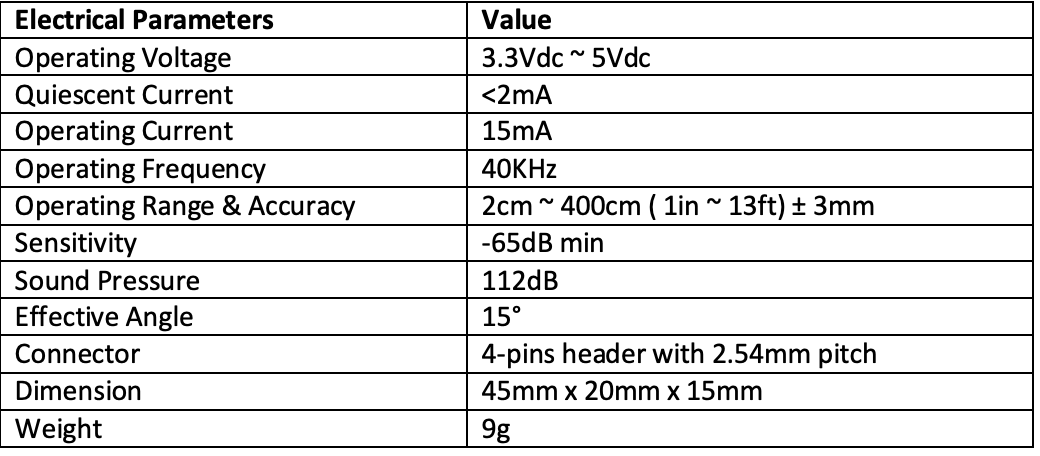
\includegraphics[width=\linewidth]{images/electrical/hc_sr04.png}
    \caption{HC-SR04 specifications table }
    \label{fig:hcSr04_specifications}
\end{figure}


The timing diagram, Figure~\ref{fig:hcSr04_schematic_timing}  is shown below. You only need to supply a short 10uS pulse to “Trigger Input”
pin to start the ranging. The module will send out 8-cycles burst of ultrasound at 40KHz and raise its “Echo” 
6 pin, refer to Figure~\ref{fig:hcSr04_schematic_mcu}. The echo is a distance object that is pulse width and the range in proportion. You can
calculate the range through the time interval between sending trigger signal and receiving echo signal.
Formula: µS / 58 = centimeters or µS / 148 =inch
or: the range = high level time * sound velocity (340m/s) / 2; 

\begin{figure}[H]
    \centering
    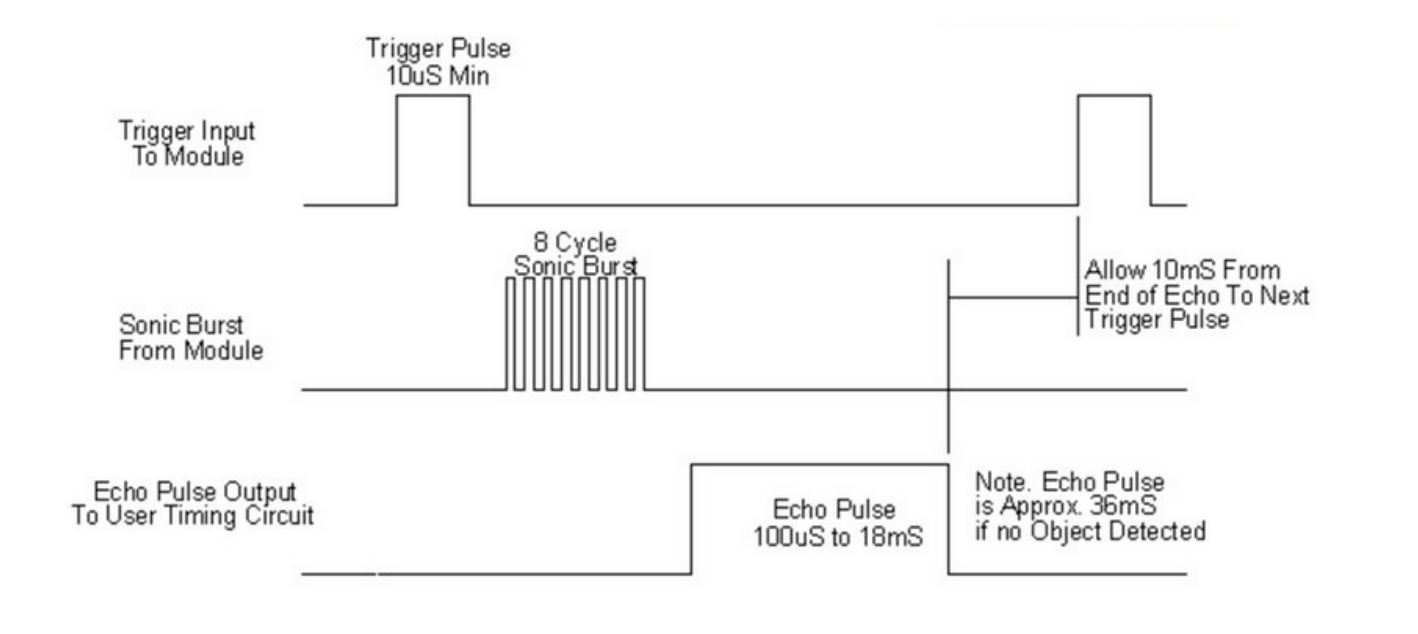
\includegraphics[width=\linewidth]{images/electrical_schematics/hcsr04_timing.png}
    \caption{HC-SR04 timing schematic diagram}
    \label{fig:hcSr04_schematic_timing}
\end{figure}

\begin{figure}[H]
    \centering
    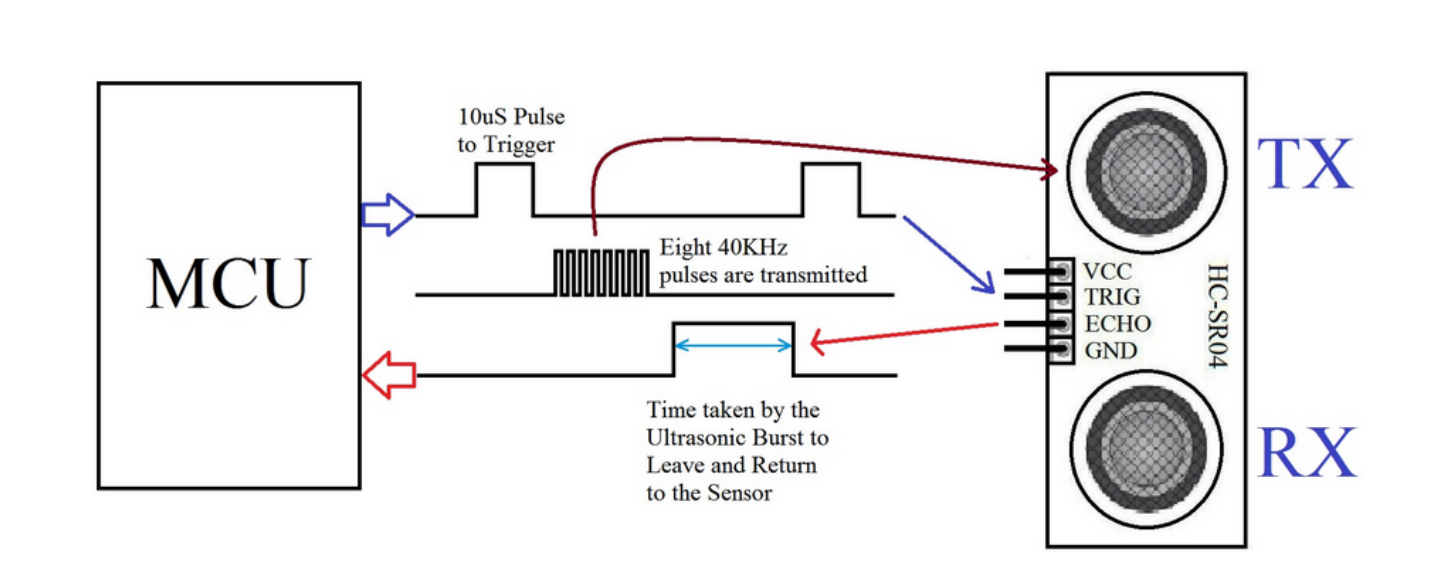
\includegraphics[width=\linewidth]{images/electrical_schematics/hcsr04_mcu.png}
    \caption{HC-SR04 timing schematic diagram}
    \label{fig:hcSr04_schematic_mcu}
\end{figure}


\subsection{IMU sensor: MPU 9250}
\par
The MPU-9250 is a compact 9-axis motion tracking sensor developed by \href{https://invensense.tdk.com/en-us}{TDK InvenSense}. 
It integrates three sensing components into a single chip:\verb|accelerometer, gyroscope, magnetometer|.
This module is more superior than older IMU sensor generation like MPU 6050. By integrated 9 axis for 3 sensors in 1 module, it helps
simplify electrical system while provide the same functions that requires multiple modules. This combination enables full 9 degrees of freedom 
(9-DoF) motion tracking, making the MPU-9250 suitable for applications requiring orientation, motion detection, and navigation.


\begin{figure}[H]
    \centering
    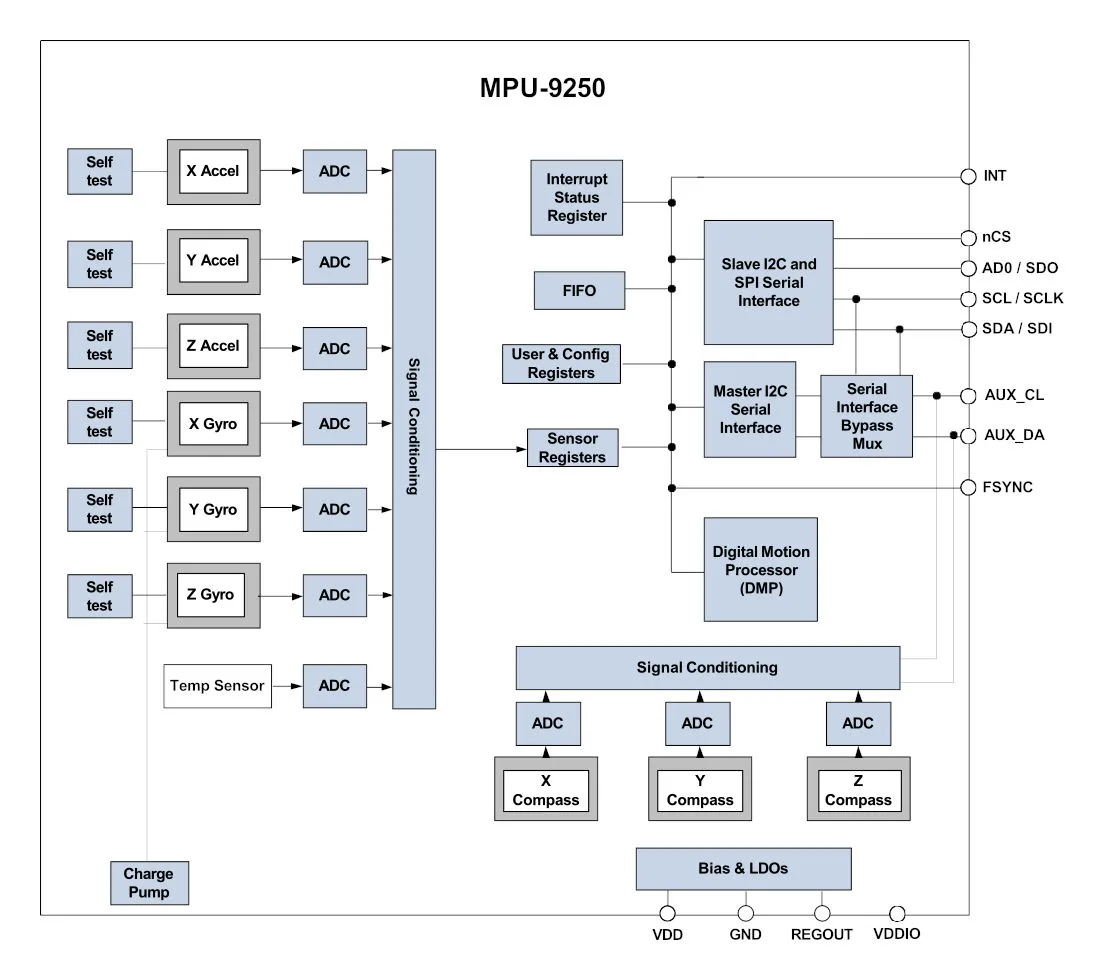
\includegraphics[width=\linewidth]{images/electrical_schematics/mpu9250-block-diagram.png}
    \caption{MPU-9250 block diagram, more information can be found in this \href{https://cdn.sparkfun.com/assets/learn_tutorials/5/5/0/MPU9250REV1.0.pdf}{datasheet}, announced by TDK InvenSense}
    \label{fig:mpu9250_diagram}
\end{figure}


\textbf{Overview}
\par
In this part, we not dive into detailed and technical specification, we only focus 3 main general 
functions are: \textbf{gyroscope, accelerometer and magnetometer}

\vspace{1.5em}
\par
The MPU-9250 consists of three independent vibratory MEMS rate gyroscopes, which detect rotation about
the X-, Y-, and Z- Axes. When the gyros are rotated about any of the sense axes, the Coriolis Effect causes
a vibration that is detected by a capacitive pickoff. The resulting signal is amplified, demodulated, and filtered
to produce a voltage that is proportional to the angular rate. This voltage is digitized using individual on-chip
16-bit Analog-to-Digital Converters (ADCs) to sample each axis. The full-scale range of the gyro sensors
may be digitally programmed to ±250, ±500, ±1000, or ±2000 degrees per second (dps). The ADC sample
rate is programmable from 8,000 samples per second, down to 3.9 samples per second, and user-selectable
low-pass filters enable a wide range of cut-off frequencies.

\vspace{1.5em}
\par
The MPU-9250’s 3-Axis accelerometer uses separate proof masses for each axis. Acceleration along a
particular axis induces displacement on the corresponding proof mass, and capacitive sensors detect the
displacement differentially. The MPU-9250’s architecture reduces the accelerometers’ susceptibility to
fabrication variations as well as to thermal drift. When the device is placed on a flat surface, it will measure
0g on the X- and Y-axes and +1g on the Z-axis. The accelerometers’ scale factor is calibrated at the factory
and is nominally independent of supply voltage. Each sensor has a dedicated sigma-delta ADC for providing
digital outputs. The full scale range of the digital output can be adjusted to ±2g, ±4g, ±8g, or ±16g


\vspace{1.5em}
\par 
The 3-axis magnetometer uses highly sensitive Hall sensor technology. The magnetometer portion of the IC
incorporates magnetic sensors for detecting terrestrial magnetism in the X-, Y-, and Z- Axes, a sensor driving
circuit, a signal amplifier chain, and an arithmetic circuit for processing the signal from each sensor. Each
ADC has a 16-bit resolution and a full scale range of ±4800 µT.


\subsection{Buck converter: LM2596}

Sensors used in MAVEN-01 like MPU, DHT11 work stable at 3.3V, but the power supply provide 6V, which mean if we connect it
directly to sensors, sensors will be damaged, so we need \href{https://www.ti.com/lit/ds/symlink/lm2596.pdf}{LM2596} 
to lower the voltage.


\begin{figure}[H]
    \centering
    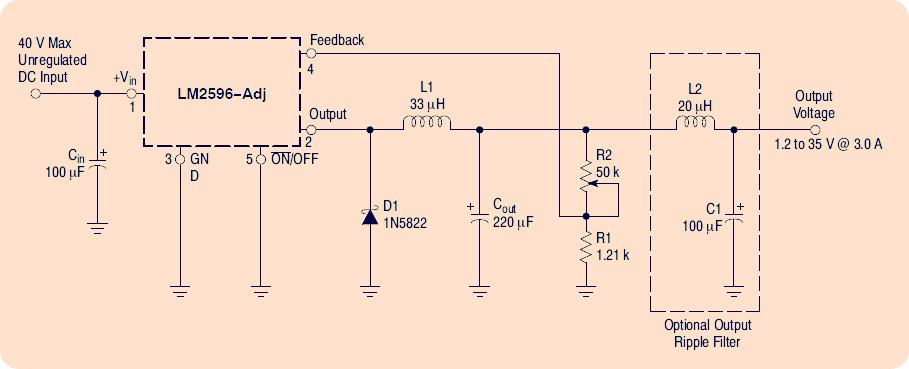
\includegraphics[width=\linewidth]{images/diagram/LM2596.png}
    \caption{LM2596 block diagram, more information can be found in this \href{https://www.alldatasheet.com/datasheet-pdf/view/543770/TI1/LM2596.html}{datasheet}, announced by Texas Instruments}
    \label{fig:lm2596_diagram}
\end{figure}

\begin{figure}[H]
    \centering
    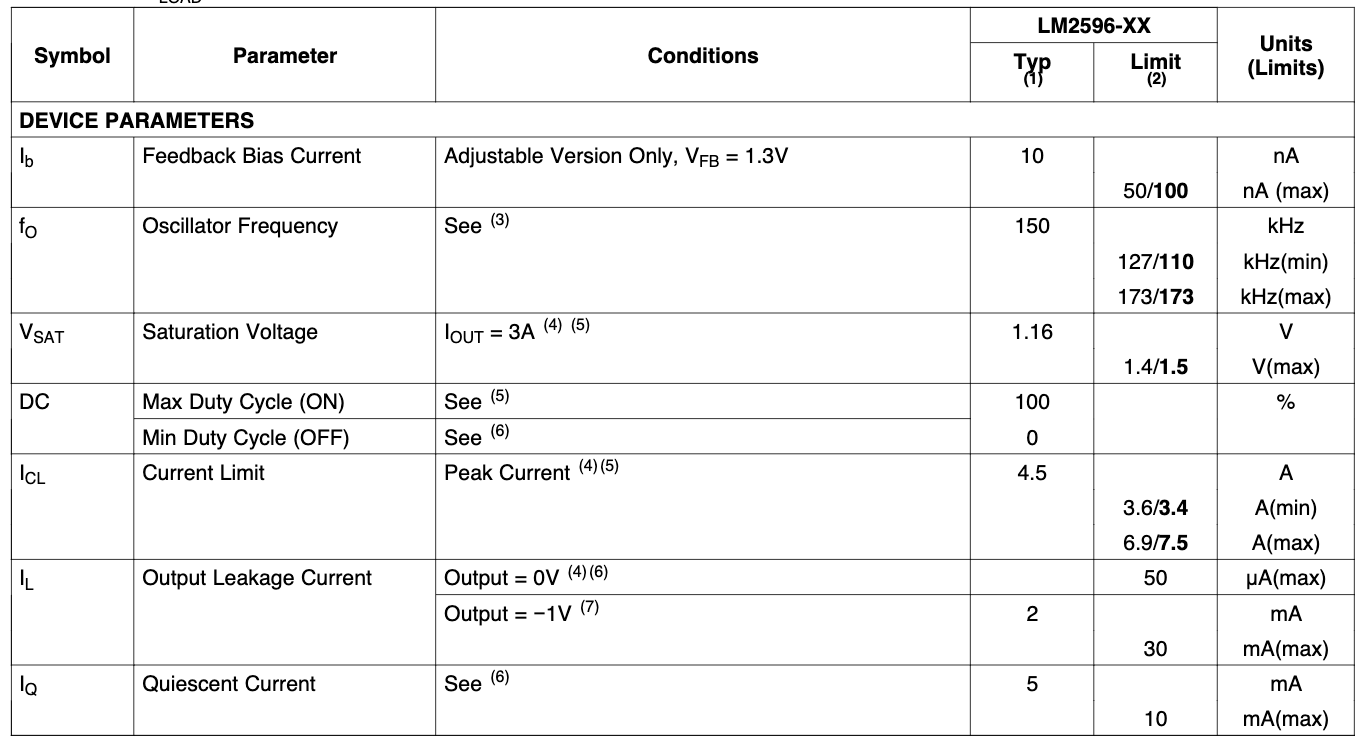
\includegraphics[width=\linewidth]{images/information/lm2596_spec.png}
    \caption{LM2596 specifications table}
    \label{fig:lm2596_tables}
\end{figure}



\subsection{Power source}
In Diagram~\ref{fig:maven_01_system_architecture}, MAVEN-01 was designed with three separate power sources. 
This design lays the groundwork for stable operation and minimizes chain-reaction failures. For instance, if any part of MAVEN-01 fails 
for any reason, we can easily identify the cause and immediately disconnect the faulty part from the system without shutting down 
the entire system.

\vspace{1em}
\par
For the microcontroller board, we use a 9V box battery since the Wemos D1 R32 board supports a voltage range 
from 9V to 12V. For all sensors, we use four AA batteries with a total output of 6V, but we use an LM2596 buck converter to reduce the voltage
to 3.3V in order to avoid damaging the sensors. For the motor power supply, we use two 18650 3.7V batteries with a high current rating of 13A and a total capacity of 5200mAh,
which is more than enough for 6--8V TT gear motors. However, when MAVEN-01 is upgraded, we will not need to replace the entire power supply system, making it more cost-efficient.























